% ERA-Großpraktikum: Entwickleranleitung -- Erweiterung

\section{Erweiterung}
\label{sec:extension}

Der folgende Abschnitt soll Anhaltspunkte zur Erweiterung des Simulators bieten.
Eine Erweiterung kann entweder ein neues Assembler-Paket (also die Unterstützung
einer neuen Assembler-Sprache, z.B. Intel-386\todo{Stimmt der Name?}) oder ein
neues Modul (''Extension'') für das bereits vorhandene Assembler-Paket RISC-V
(z.B. das Modul RV32F) sein. Des Weiteren ist es auch möglich, weitere
Komponenten in der GUI zu ergänzen.\\

Da der Simulator für mehrere Assembler-Pakete konzipiert worden ist, müssen
große Teile der Benutzeroberfläche und auch der Grundstruktur nicht neu
geschrieben bzw. verändert werden. Vielmehr kommt es darauf an, das Konzept der
bereits vorhandenen Teile zu verstehen und anzuwenden.\\

\subsection{Übersicht zur Architektur}

Um zu verstehen, wo die Erweiterung im Konzept einzuordnen ist, und welche
Klassen zu implementieren sind, sollte man den Prozess verstehen, wie genau ein
Assembler-Paket geladen und angesprochen wird. Einen groben Überblick bietet
folgendes Diagramm. Die Namen der Komponenten finden sich so nicht im Code
wieder, sie dienen lediglich als Oberbegriff für eine ganze Reihe von Klassen
und -strukturen die grob die selbe Aufgabe haben.

\begin{figure}
	\centering
	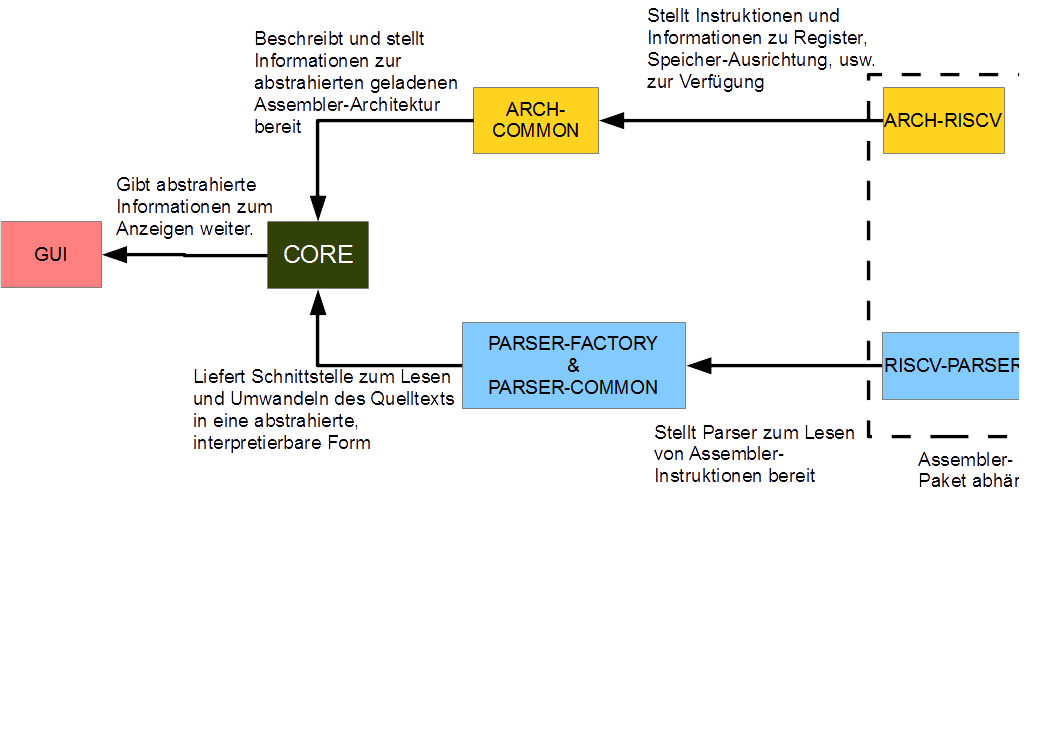
\includegraphics[scale=0.5]{charts/extension-overview.png}
	\label{dev-manual-extension-overview}
\end{figure}

\todo[inline]{Besseres Bild kommt noch (Erik)}

Nach der Auswahl des Assembler-Pakets durch den Benutzer in der
Benutzeroberfläche werden ausgewählter Architekturname, gewählte Extensions und
der gewählte Parser an den Core übergeben. Dieser lädt über Arch-Common Daten
des Pakets und seinen Extensions, anschließend wird der passende Parser über die
Parser-Factory erzeugt. Die Daten von Arch-Common enthalten zum Einen
standardisierte, abstrahierte Informationen zum geladenen Paket (z.B. Länge,
Anzahl, Funktion und Name von Registern, Speicher-Ausrichtung, Endianness, ...)
und zum Anderen Zugriff auf Factories zur Erzeugung von Instruktionsknoten.\\
Soll jetzt ein Quelltext eingelesen und ausgeführt werden, bekommt der Core den
Text und gibt diesen an die geladene Parser-Implementierung weiter. Diese
Implementierung wandelt das Programm in eine paket-unabhängige Darstellung
mithilfe eines Syntaxbaumes um. Die Knoten des Syntaxbaums kann der Parser dabei
über die Knoten-Factories der geladenen Architektur beziehen. Die
paket-unabhängige Darstellung wird daraufhin vom Core ausgeführt. Alle Effekte
auf Register und Speicher passieren in einer abstrahierten Art, so dass die
Benutzeroberfläche Veränderungen anzeigen kann, ohne die konkrete
Implementierung der Architektur zu kennen.\\

Es sind also nur diejenigen Teile zu implementieren, die im Diagramm gestrichelt
umrandet sind. Es muss eine Architekturdefinition inklusive Implementierungen
der einzelnen Instruktionen und ein Parser für diese geschrieben werden.

\subsection{Implementierung des Architektur-Teils}

Wie schon in \autoref{dev-manual-extension-overview} zu sehen, gibt es einen
Teil, der bei jedem Paket existiert und die entsprechende Abstraktion nach außen
(also Core und GUI) aufbaut. Der Architektur-Teil lässt sich weiter
untergliedern in Definition und Eigenschaften des Assembler-Pakets,
Implementierung des Verhaltens der Instruktionen und das Bereitstellen dieser
für den Parser zum Bau eines Syntaxbaumes.

\begin{figure}[ht]
	\centering
	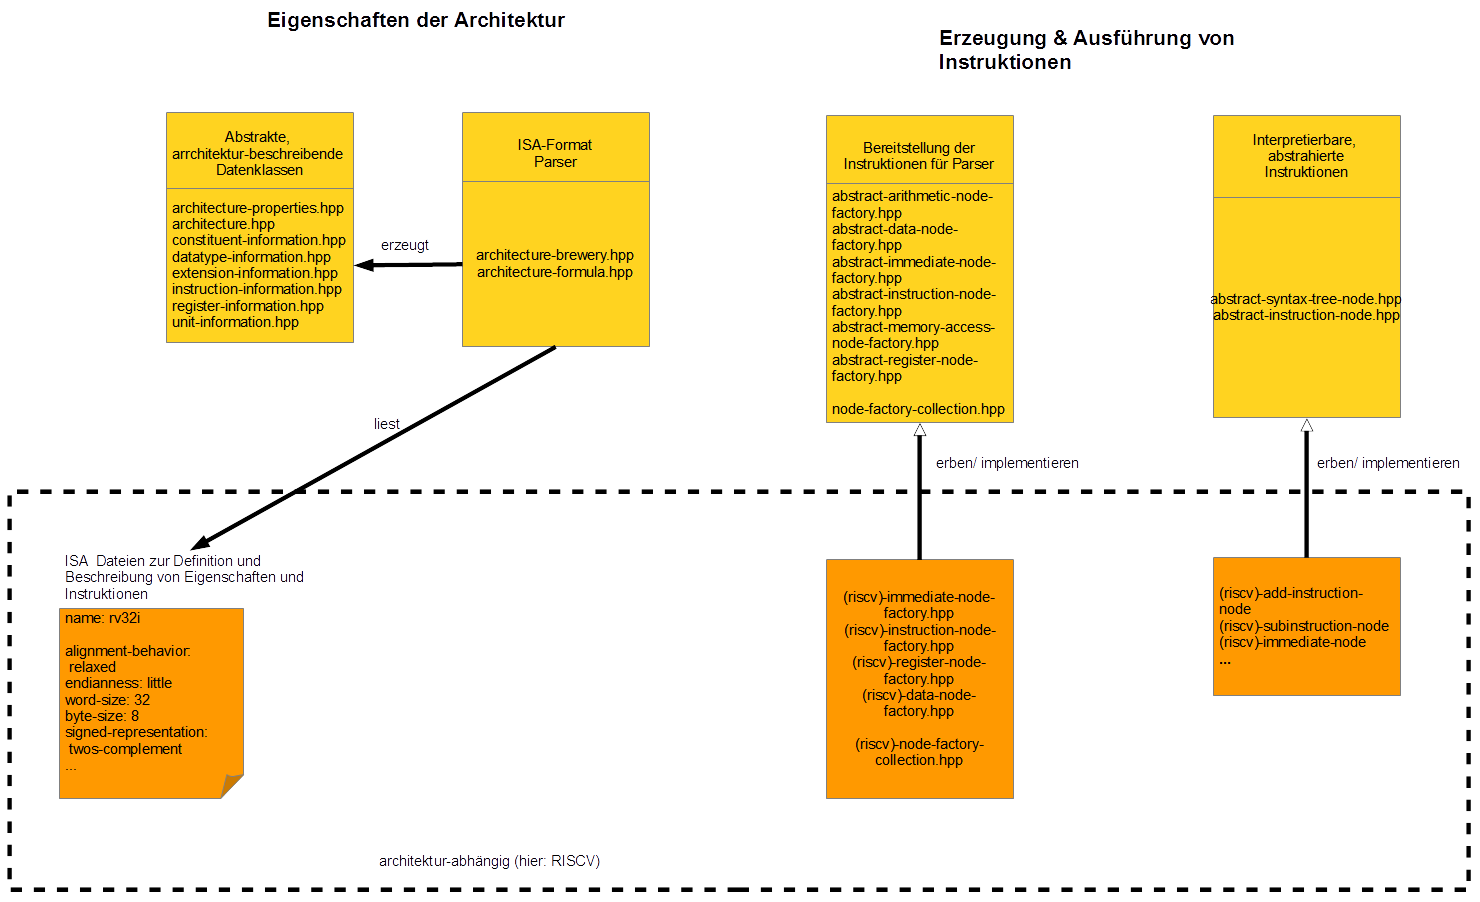
\includegraphics[scale=0.45]{charts/extension-arch.png}
\end{figure}

\subsubsection{Definition und Eigenschaften des Assembler-Pakets}

Für diesen Bereich ist keine Zeile Code nötig. Da eine Implementierung von
Datenklassen zur Beschreibung der Eigenschaften sich inhaltlich, aber nicht
strukturell unterscheiden wird, muss für eine Erweiterung lediglich eine
Beschreibungsdatei im ISA-Format\todo{Verweis zur Beschreibung der ISA-Sprache}
erstellt werden. Die Datei wird in YAML geschrieben, dann per Script nach JSON
übersetzt und in den \texttt{isa} Ordner des Simulators abgelegt. Dort wird dann
bei Programmstart und entsprechender Auswahl die JSON Datei eingelesen und
bereits vorhandene Datenklassen mit Werten befüllt. Speicherort und Name der
ISA-Dateien wird so erwartet: Innerhalb des ISA Ordners liegt ein Ordner mit
Namen der Architektur. Innerhalb dieses Ordners liegen Ordner mit Namen der
Extensions (auch die Basis bzw. Grundversion ist eine Extension), in denen
wiederum befindet sich die JSON Datei \texttt{config.json} (und der
Bequemlichkeit halber auch das YAML Gegenstück). Beispiel: Die
Assembler-Architektur \texttt{myArch} hat ein Basismodul \texttt{arch\_base} und
eine Erweiterung \texttt{arch\_fancy}:

\begin{lstlisting}
era-gp-sim -- isa -- riscv.isa -- ...
                  |- test.isa  -- ...
                  |- myArch.isa   -- arch_base -- config.json
                                  |          \- config.yaml
                                  \- arch_fancy -- config.json
                                                \- config.yaml
\end{lstlisting}
In den ISA-Files werden folgende Eigenschaften definiert:

\begin{itemize}
	\item Name, Wortgröße, Endiannes des Pakets
	\item Name, Größe, Funktion (Programmzähler, Flag, etc.) und Startwert der Register
	\item Name, Format der Assemblierung, Opcode jeder Instruktion
	\item (Optional) Definition von Makros (sofern Makros vom Parser unterstützt werden), die der Benutzer verwenden kann
\end{itemize}

\subsubsection{Implementierung der Instruktionen}
\label{extension-arch-ast}

Der zentrale und auch für den Nutzer sichtbare Teil einer neuen Architektur sind
die neuen Instruktionen. Eine konkrete Instruktion also z.B. \texttt{addi x1,
x0, 0x45 (riscv)} wird intern als Syntaxbaum dargestellt. Der Parser verwandelt
jede Zeile Quelltext in einen Baum. Diese Liste an Bäumen repräsentiert dann das
ausführbare Programm. Alle Knoten des Baumes erben von einer Oberklasse, der
\texttt{AbstractSyntaxTreeNode}.\\ Die grundlegende Idee ist, dass die
Ausführungseinheit nur eine bestimmte Methode (nämlich
\texttt{AbstractSyntaxTreeNode::getValue(...)}) zur Ausführung der, durch den
Baum repräsentierten, Instruktion aufruft. Die Wurzel macht dementsprechend
rekursive Aufrufe an die Kind- bzw. Operandenknoten. Das hat den Vorteil, dass
eine Instruktion mit selbem Verhalten, die z.B. einmal ein Register und einmal
eine Konstante erwartet, nicht zweimal implementiert werden muss. Die
eigentliche Gestalt (also Register- oder Konstantenknoten) wird durch eine
gemeinsame Oberklasse versteckt. Das bedeutet natürlich auch, dass zur
Validierung auch auf den Typ der Operandenknoten geachtet werden muss.\\

Da für einige Funktionen in der Benutzeroberfläche (z.B. das Anzeigen von
Hilfetexten zur richtigen Instruktion) besondere Daten gespeichert und
erreichbar gemacht werden müssen, gibt es die \texttt{AbstractInstructionNode}.
Dieses Kind von \texttt{AbstractSyntaxTreeNode} muss zwingend von der Fabrik für
Instruktionen zurückgegeben werden. Sie bildet außerdem immer die Wurzel des
Syntaxbaumes pro Befehl.\\

Zuerst betrachten wir die für jeden Knotentyp zu implementierenden Methoden der
Oberklasse \texttt{AbstractSyntaxTreeNode}. Danach wird noch auf die speziellen
Anforderungen zu Implementierungen von \texttt{AbstractInstructionNode}
eingegangen.

\begin{itemize}

  \item \texttt{MemoryValue} \textbf{getValue} \texttt{(MemoryAccess)} \\ Wird
  zur Ausführung des Syntaxbaumes aufgerufen. Die verschiedenen Knotentypen
  geben dann ihrer Rolle entsprechende Werte zurück. Beispielsweise gibt ein
  Registerknoten den Inhalt des Registers, ein Konstantenknoten die Konstante
  zurück.

	\item \texttt{ValidationResult} \textbf{validate}\texttt{(MemoryAccess)} \\
	Wird aufgerufen, um zur Übersetzungszeit zu überprüfen, ob die aktuelle
	Konstellation dieses Syntaxbaums eine gültige Instruktion darstellt.

	\item \texttt{ValidationResult}
	\textbf{validateRuntime}\texttt{(MemoryAccess)} \\ Wird aufgerufen, um zur
	Laufzeit (also direkt vor der Ausführung der Instruktion) zu überprüfen, ob
	dieser Syntaxbaum gültig ist. Eine Sprunginstruktion überprüft hier
	beispielsweise, ob die Sprungadresse zusammengesetzt aus Registerwert und
	Marke gültig, d.h. ins Textsegement zeigt und richtig angeordnet ist.

	\item \texttt{MemoryValue} \textbf{assemble}\texttt{()} \\ Gibt den Knoten in
	assemblierter Form zurück. Ein Registerknoten x5 gibt z.B. \texttt{00101}
	(also 5 als Binärzahl der Länge n), ein Konstantenknoten gibt seinen Wert
	zurück. Der Instruktionsknoten (die Wurzel) gibt anschließend die
	zusammengefügte, komplette assemblierte Instruktion zurück.

\end{itemize}

Anforderungen an \texttt{AbstractInstructionNode}

\begin{itemize}

  \item \texttt{MemoryValue} \textbf{getValue} \texttt{(MemoryAccess)} Hier
  führt die Implementierung einer Instruktion das Verhalten der Instruktion aus.
  Als Rückgabewert erwartet die Ausführungseinheit die Adresse des als nächstes
  auszuführenden Befehls. Da die Ausführungseinheit nicht weiß, welches Register
  den Programmzähler repräsentiert, muss dieses Register zusätzlich aktualisiert
  werden. \\ Beispielsweise könnte in Pseudocode eine Additionsinstruktion
  \texttt{add rd, rs1, rs2} wie folgt implementiert werden:

\begin{lstlisting}{style=c++}
MemoryValue getValue(MemoryAccess memoryAccess) {
	assert::that (_children.count == 3)
	Value rs1 = _children[1].getValue(memoryAccess);
	Value rs2 = _children[2].getValue(memoryAccess);
	Value sum = rs1+rs2;
	Identifier regId = _children[0].getIdentifier();
	memoryAccess.putRegisterValue(regId, sum);
	addToProgramCounter(4);
	Value pc = memoryAccess.getRegisterValue("pc");
	return pc;
	}
\end{lstlisting}

	Durch die allgemein gehaltenen Operanden, kann der selbe Code auch für
	\texttt{add rd, rs1, immediate}, für \texttt{add rd, rs1, [rs2]} oder
	\texttt{add rd, rs1, [k*rs2+d]} verwendet werden\footnote{Der []-Operator
	deutet einen Speicherzugriff änhlich zur Intel 386 Syntax an}.

  \item \texttt{Translateable} \textbf{getInstructionDocumentation} \texttt{()}
  Gibt einen übersetzbaren Hilfetext für den aktuellen Befehl zurück. Der
  Hilfetext wird dann gegebenenfalls in der Hilfetextkomponente der
  Benutzeroberfläche angezeigt. Ob der Text erst bei Aufruf erzeugt, im Knoten
  gespeichert oder aus einer Tabelle mit vorgefertigten Texten entnommen wird,
  ist der Implementation überlassen. RISC-V verwendet Letzteres.

\end{itemize}

\subsubsection{Bereitstellen der Instruktionen für den Parser}
\label{extension-arch-factories}

Der Parser baut beim Übersetzen aus jedem Befehl einen Syntaxbaum. Der Parser
kennt aber die genauen Signaturen und damit die Implementierungen der
Syntaxbaumknoten nicht. Um zur Laufzeit trotzdem die richtige
Knotenimplementierung zu erzeugen, verwenden wir hier das
Factory-Design-Pattern\footnote{https://de.wikipedia.org/wiki/Fabrikmethode}. Da
der Parser nur die syntaktische Bedeutung eines Symbols kennt, nicht aber seine
Semantik (also das Verhalten, die Implementierung), ruft der Parser die passende
Fabrik auf, die dann eine semantisch passende Implementierung instanziiert und
zurückgibt. Der Parser kann aufgrund z.B. der Position des Symbols auf seine
syntaktische Rolle schließen. Das erste Word, das keine Direktive oder Marke
ist, muss der mnemotechnische Befehl sein; der Ausdruck danach muss der erste
Operand sein, usw. \\
Welche Arten von Knoten-Fabriken es gibt wurde bereits in
\autoref{module-arch-node-factory} beschrieben. Wird eine Fabrik nicht
implementiert (z.B. bei RISC-V \texttt{arithmetic-node-factory}) ist das in
Ordnung, solange der Parser die Fabrik nicht verwendet. Da aber sowohl Parser
als auch Fabrik-Implementierung in einer Erweiterung entstehen müssen, sollte
das kein Problem darstellen. Jede Fabrik-Klasse erzeugt genau eine Art von
Knoten (siehe \autoref{module-arch-ast-node-types}).\\

Der Parser hat wegen der Abstraktion, die eine Fabrik bietet, keine Kenntnis
darüber, ob eine Implementierung einer bestimmten Instruktion vorhanden ist. Die
Entscheidung ist jedoch sehr wichtig, da im Fall einer fehlenden Implementierung
der Parser einen Übersetzungsfehler generieren muss, da eine Instruktion des
Nutzerprogramms nicht existiert.\\
Da sowohl die Verwendung der Fabriken im Parser, als auch die Implementierung
der Fabriken im Bereich der Erweiterung liegt, kann für diese Problemstellung
eine beliebige Lösung gefunden werden. Es gibt dahingehend keine strikte
Regel.\\
Die Implementierung der RISC-V Module inklusive des RISC-V Parsers verwenden die
Rückgabe eines \texttt{nullptr} zur Anzeige einer fehlenden Instruktion. Genauso
möglich ist z.B. auch das Werfen einer Exception.

Da das Verwalten von bis zu sechs Fabriken für eine Parserimplementierung
unübersichtlich wird, gibt es eine einzige Instanz
(\texttt{NodeFactoryCollection}) die das Interface der einzelnen Fabriken
spiegelt und Aufrufe entsprechend weiterleitet. Die Parserimplementierung muss
nur die \texttt{NodeFactoryCollection}-Instanz verwalten.\\
Die NodeFactoryCollection wird automatisch beim Laden der Architektur aus den
ISA-Dateien erzeugt und dem Architektur-Objekt als Member mitgegeben. Damit das
funktioniert muss in \texttt{arch/commons/node-factory-collection-maker.cpp} in
der Funktion \texttt{CreateFor} für die neue Architektur eine passende
NodeFactoryCollection zurückgegeben werden.\\
Für RISC-V haben wir im riscv-namespace eine NodeFactoryCollection mit den
RISC-V Implementierungen der benötigten Fabriken definiert (siehe
\texttt{arch/riscv/factory-types.hpp}).

\subsection{Erweiterung der GUI}
Soll eine neue Komponente zur GUI hinzugefügt werden, gibt es mehrere
Entscheidungen zu treffen. Die Komponente kann etwas bestehendes, wie die
Ausgabe, erweitern oder komplett neu sein. in diesem Fall gilt es noch zu
klären, ob sie Projektspezifisch, wie Speicher oder Register, ist oder auf das
ganze Programm, also außerhalb der TabView wie die Menubar, bezogen werden soll.

\subsubsection{Erweiterung bestehender Komponenten}
Das Erweitern bestehender Komponenten ist vergleichsweise einfach. Hier gilt es,
in der entsprechenden C++-Datei nachzuschlagen. Ist, wie bei der Ausgabe, nur
eine für die gesamte Komponente angelegt, müssen hier etwaige Attribute und
Methoden ergänzt werden. Ist dagegen für jeden einzelnen Teil eine eigene Datei
angelegt, so sollte auch für die Erweiterung eine ergänzt werden. Man beachte,
dass es wahrscheinlich nötig sein wird, die Instanzen zum \texttt{QQMLContext}
hinzuzufügen.\\
In QML sind Komponenten, die mehrere eigene Module besitzen, üblicherweise in
einer TabView dargestellt. Es muss also nur ein Tab in der Hauptdatei der zu
erweiternden Komponente ergänzt werden. Die eigentliche Definition sollte in
einer eigenen Datei in einem neuen Unterverzeichnis erfolgen. Im Allgemeinen
sollte auch auf ein Einstellungsfenster, die entsprechende Funktion und die
Themes geachtet werden. Um zu erkennen, ob dies nötig ist, beachte man die
anderen Module.

\subsubsection{Neue Komponenten}

Auch das Hinzufügen neuer Komponenten gestaltet sich nicht besonders schwierig.
Für den QML-Teil ist Folgendes zu tun: Im Ordner \texttt{ui/Components} ein
neuer Ordner angelegt werden. Dort werden alle neuen Dateien der Erweiterung
abgelegt. Außerhalb dieses Ordners muss nur die Datei
\texttt{ui/SplitviewItem.qml} modifiziert werden. Hier muss in der ComboBox der
entsprechende Name eingetragen werden, in den Variablen \texttt{model} und
\texttt{usualList}. Außerdem muss unten im Loader der Pfad der Hauptdatei
hinzugefügt werden, am gleichen Index wie der Name in der ComboBox. Des weiteren
sei bemerkt, dass jede neue Komponente eine Variable
\texttt{hasComponentSettings} benötigt.\\
Der C++-Teil wird einfach unter \texttt{ui} abgelegt. Auch ein Header sollte im
entsprechenden Verzeichnis vorhanden sein. Soll die Komponente für jedes Projekt
einzeln verwendet werden, so wird eine neue Instanz der C++-Klasse in der
entsprechenden Instanz der Klasse \texttt{GuiProject} hinterlegt. Von dort kann
man auch den \texttt{QQmlContext} bekommen. Dieser ist zwingend nötig, wenn aus
QML auf die C++ Instanz zugegriffen werden soll. Ist die neue Komponente dagegen
für alle Projekte gleich, so verwende man die \texttt{Ui} Klasse. Bei der
Programmierung der neuen C++-Klasse sollte der Abschnitt zur Kommunikation der
Module beachtet werden, siehe \autoref{gui-kommunikation}.

 \subsection{Weitere Anmerkungen}

 \subsubsection{Konzept zur Lokalisierung (Übersetzbarkeit von angezeigten Texten)}

 Eine Anforderung an den Simulator ist die Möglichkeit, jeden angezeigten Text
 zu lokalisieren. Zum Zeitpunkt der ersten Version des Simulators existiert
 lediglich eine englische Version der Hilfetexte. Damit der Simulator auch in
 Zukunft vollständig übersetzbar bleibt, muss auch die Erweiterung um eine neue
 Architektur einige Maßnahmen treffen.\\

 Wir haben uns dazu entschieden die Übersetzungsfunktionalitäten von Qt zu
 verwenden\footnote{http://doc.qt.io/qt-5/i18n-source-translation.html}. Kurze
 Zusammenfassung über das Konzept von Qt:\\
 Diejenigen Nachrichten und Texte, die zu irgendeinem Zeitpunkt (sei es
 Initialisierung einer GUI-Komponente oder z.B. generierte Hilfetexte) dem
 Benutzer angezeigt werden sollen, \textbf{müssen} im Quelltext als
 Stringliteral (\texttt{char$\lbrack \rbrack$} oder \texttt{char*}, nicht jedoch
 \texttt{std::string}) definiert und mit einem speziellen
 Makro\footnote{\texttt{QT\_TRANSLATE\_NOOP} und ähnliche} markiert werden.
 Jeder Text, der angezeigt wird, muss vorher durch eine der verschiedenen
 \texttt{translate}-Funktionen übersetzt werden.\\

 Die obigen Maßnahmen müssen zwingend durchgeführt werden, denn sollte eine
 Lokalisierung aller Texte vorgenommen werden wollen, wird das wie folgt
 ablaufen:\\

 Ein Unterprogramm von QtLinguist (lupdate) sucht im \textbf{Quelltext} des
 Simulators nach allen zur Übersetzung markierten Stringliteralen und fügt diese
 in eine Tabelle ein. Diese Tabelle wird anschließend mit QtLinguist übersetzt
 und erzeugt sogenannte Translateable Source-Dateien. Diese Dateien, z.B. die TS
 für deutsche Lokalisierung, müssen dann mit dem Simulator ausgeliefert werden
 und werden beim Start durch die Qt-Library geladen und angewendet.\\

 Findet die Qt-Library aber keine solche TS-Dateien (wie zum Zeitpunkt der
 ersten Version der Fall), dann greift sie auf die Rückfalllösung -- die
 Stringliterale im Quellcode -- zurück\footnote{Für ausfühlichere Informationen
 siehe http://doc.qt.io/qt-5/qtlinguist-index.html}.\\

 Jetzt ist klar, wieso keine Texte des Typs \texttt{std::string} oder zur
 Laufzeit zusammengebaute Texte verwendet werden dürfen. lupdate könnte sonst
 den Text nicht (vollständig) in die Übersetzungstabelle einfügen und die
 Übersetzung klappt nicht mehr.\\

 Zur Kapselung eines potentiell übersetzbaren Texts gibt es die Klasse
 \texttt{Translateable} (zu finden in \texttt{commons/translateable.hpp}). Sie
 enthält Methoden zum Qt-konformen Zusammenfügen von Texten und kann nur durch
 Stringliterale erzeugt werden, um Fehler vorzubeugen.
